\subsection{Kernel-independenet fast multipole method}

The fast multipole method (\fmm) is an algorithm that can reduce the quadratic time and space complexity of such matrix-vector multiplication down to $\mathcal{O}(N)$.
In the context of \fmm, $\{\mathbf{x}_i\}$ and $\{\mathbf{y}_j\}$ in equation ? are often referred to as the set of targets and sources respectively, with $\{q_j\}$ representing the source densities (charges).
The goal of \fmm is to efficiently compute the potential at $N$ targets $\{s_i\}$ induced by all $N$ sources and the kernel function $g$.

\fmm builds upon two fundamental ideas: (1) approximating the far-range interactions between distant clusters of sources and targets using low-rank methods, while computing the near-range interactions exactly, and (2) partitioning the domain using a tree structure to maximize the far-range portion in the computation.

\begin{figure}
    \centering
    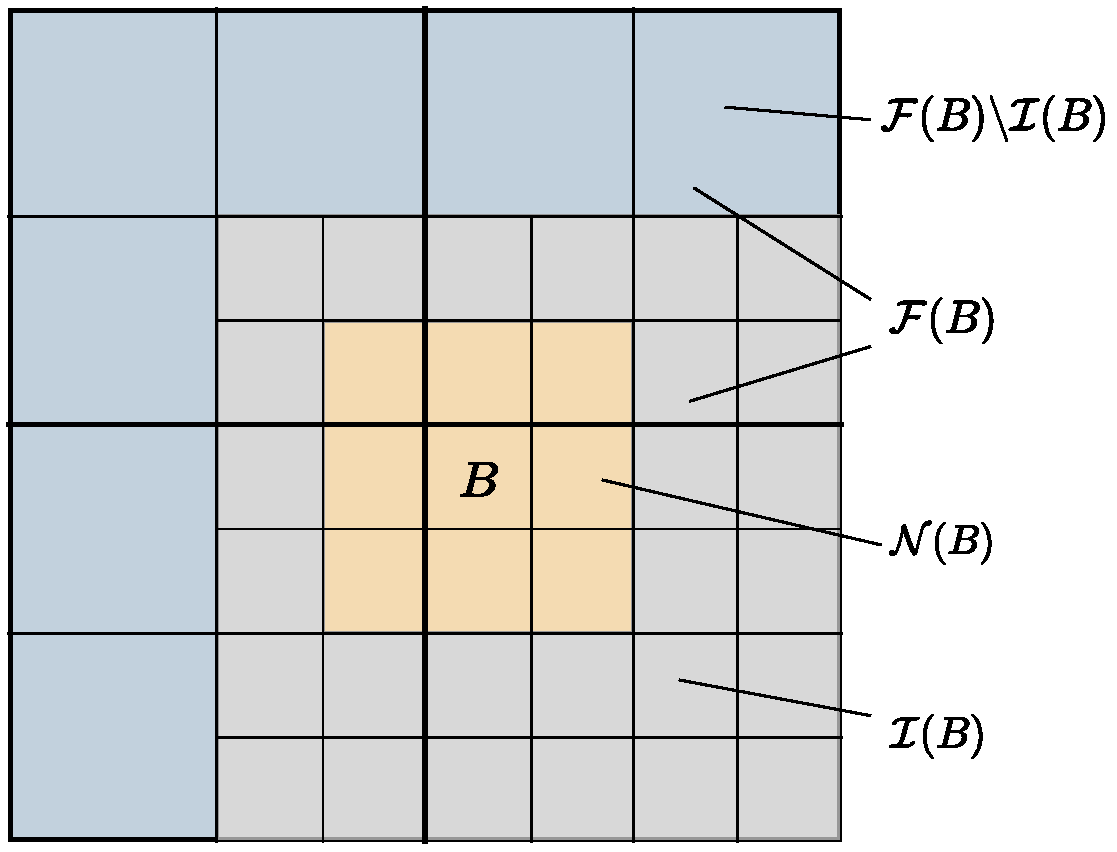
\includegraphics[width=0.8\linewidth]{near_far_decomposition.pdf}
    \caption{An example of a 3-level quadtree.}
    \label{fig:near_far_decomp}
\end{figure}

To construct the octree, we first create a cube that encloses all bodies and then recursively subdivide the domain until each cube at the finest level only contains a constant number of bodies.
Figure \ref{fig:near_far_decomp} depicts a 3-level quadtree.
The potentials of targets in the node $B$ consists of three contributions: the influence from sources in the near-field of $B$: $\mathcal{N}(B)$, in the interaction list of $B$: $\mathcal{I}(B)$ and in the rest of the domain.
$B$'s near-field includes $B$ and its neighbors, where the interactions are computed exactly.
The remaining domain is in $\mathcal{F}(B)$, $B$'s far-field.
In $\mathcal{F}(B)$, the nodes that are the children of $B$'s parent's neighbors but are not adjacent to $B$ compose $\mathcal{I}(B)$, the interaction list of $B$, whose contributions to $B$ are approximated by low-rank methods.
The contributions from the rest of the far-field are approximated at coarser levels via $B$'s ancesters.

The classic \fmm \cite{greengard1987fast, cheng1999fast} relies on truncated analytical expansions to approximate far-field interactions, whereas its kernel-independent variant \cite{ying2004kernel} uses equivalent densities (charges) instead.
In KIFMM, each node is associated with upward and downward equivalent densities (see Figure \ref{fig:multipole_local}), the analog of multipole and local expansion in analytical \fmm.
The upward equivalent densities $q^{B,u}$ are used to approximate the influence of sources in $B$ on targets in $\mathcal{F}(B)$;
the downward equivalent densities $q^{B,d}$ are used to approximate the influence of sources in $\mathcal{F}(B)$ on sources in $B$.
To find these densities, we match the potential of equivalent densities to the potential of actual sources at the check surfaces:
%
\begin{align}
    \sum_{\mathbf{y}_{j} \in B} g\left(\mathbf{x}_{i}^{B,u}, \mathbf{y}_{j}\right) q_{j} &= \sum_{j} g\left(\mathbf{x}_{i}^{B,u}, \mathbf{y}^{B,u}_{j}\right) q^{B,u}_{j}, \quad \forall i  \\
    \sum_{\mathbf{y}_{j} \in \mathcal{F}(B)} g\left(\mathbf{x}_{i}^{B,d}, \mathbf{y}_{j}\right) q_{j} &= \sum_{j} g\left(\mathbf{x}_{i}^{B,d}, \mathbf{y}^{B,d}_{j}\right) q^{B,d}_{j}, \quad \forall i
    \label{eq:multipole_local}
\end{align}
%
, and then solve the linear systems for $\{q^{B,u}_{j}\}$ and $\{q^{B,d}_{j}\}$.
$\mathbf{x}_{i}^{B}$ and $\mathbf{y}_{j}^{B}$ denote the discretization points of the check surface and equivalent surface of $B$ respectively.

\begin{figure}
    \centering
    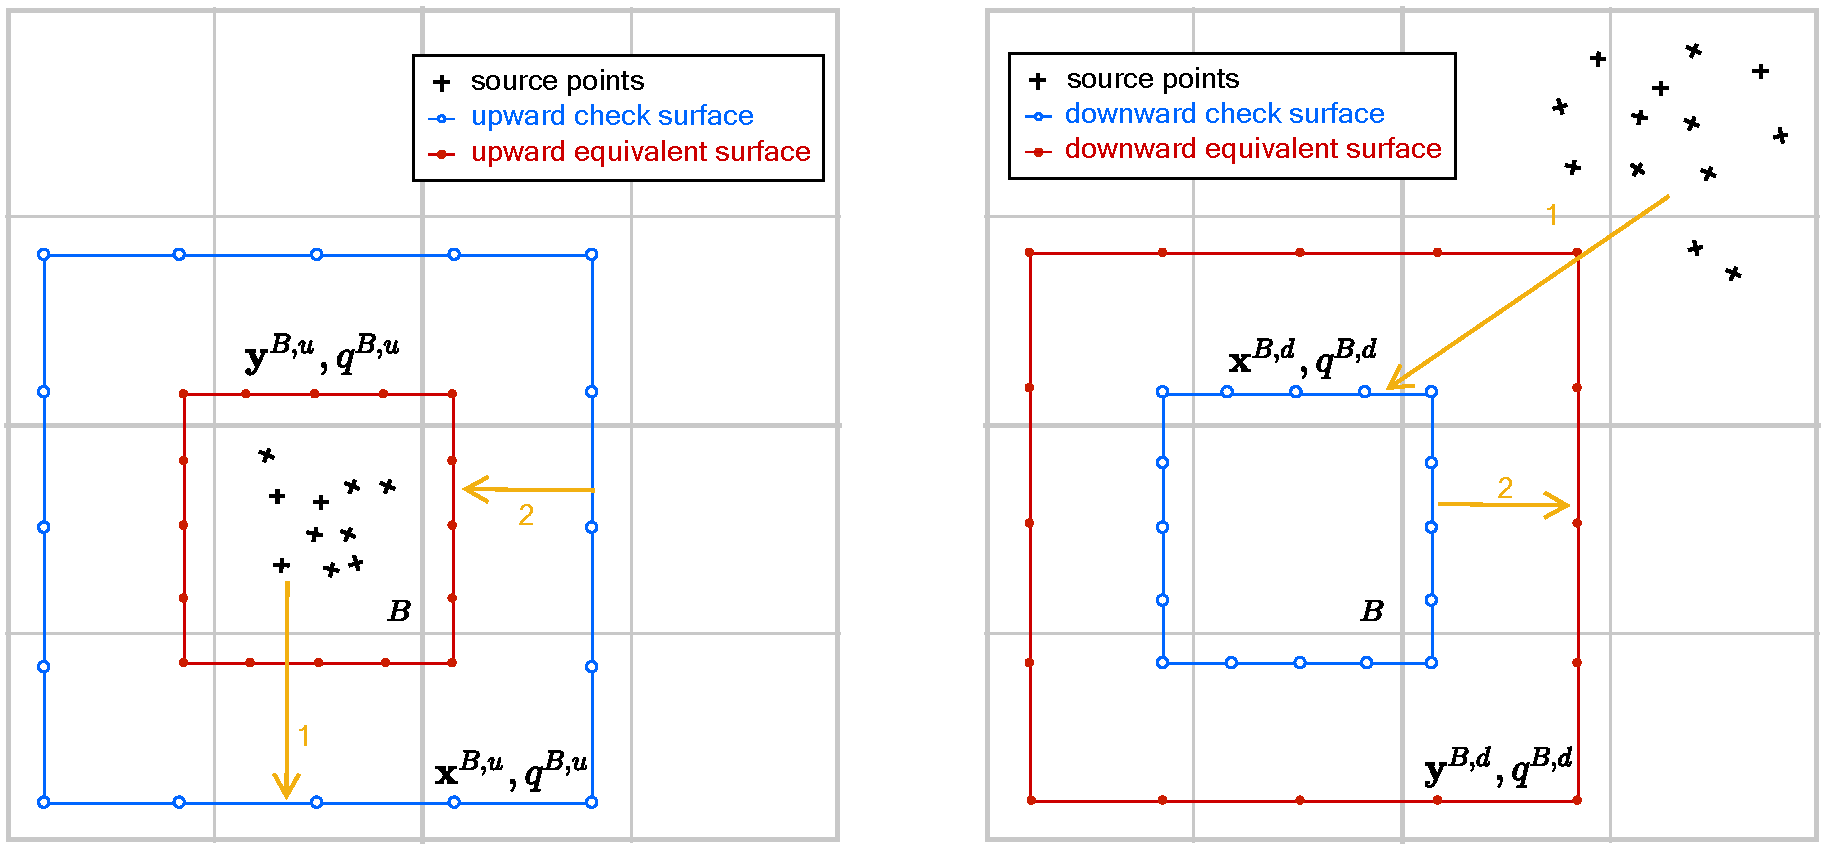
\includegraphics[width=\linewidth]{multipole_local_expansion.pdf}
    \caption{Multipole expansion (left) and local expansion (right) in KIFMM.}
    \label{fig:multipole_local}
\end{figure}

The algorithm also defines the following operators:
%
\begin{itemize}
    \item particle-to-multipole (P2M): For a leaf node $B$, compute $B$'s upward equivalent densities, \ie multipole expansion, from the sources in $B$. (Figure \ref{fig:multipole_local} left)
    \item multipole-to-multipole (M2M): For a non-leaf node $B$, evaluate $B$'s multipole expansion based on the multipole expansions of all $B$'s children. (Figure \ref{fig:translations} left)
    \item multipole-to-local (M2L): For a node $B$, evaluate $B$'s downward equivalent densities, \ie local expansion, by using the multipole expansions of all nodes in $\mathcal{I}(B)$. (Figure \ref{fig:translations} middle)
    \item local-to-local (L2L): For a non-leaf node $B$, add the contribution of $B$'s local expansion to the local expansions of $B$'s children. (Figure \ref{fig:translations} right)
    \item local-to-particle (L2P): For a leaf node $B$, evaluate $B$'s local expansion at the locations of targets in $B$.
    This step adds all far-field contribution to the potentials of targets in $B$. 
    \item particle-to-particle (P2P): For a leaf node $B$, evaluate the potential induced by all sources in $\mathcal{N}(B)$ directly.
\end{itemize}
%
As indicated by the arrows in Figure \ref{fig:translations}, translation operators in KIFMM share the same procedure: (1). evaluating the potentials on the check surface and (2). solving the equation arising from matching the potentials for the equivalent densities.

Figure \ref{fig:fmm_sketch} outlines the complete \fmm algorithm.
During the upward pass, we compute P2M at all leaf nodes and perform M2M in post-order tree traversal.
Next, we compute M2L for all nodes.
Finally, we compute L2L in pre-order tree traversal, and perform L2P and P2P at all leaf nodes during the downward pass.

\begin{figure*}
    \centering
    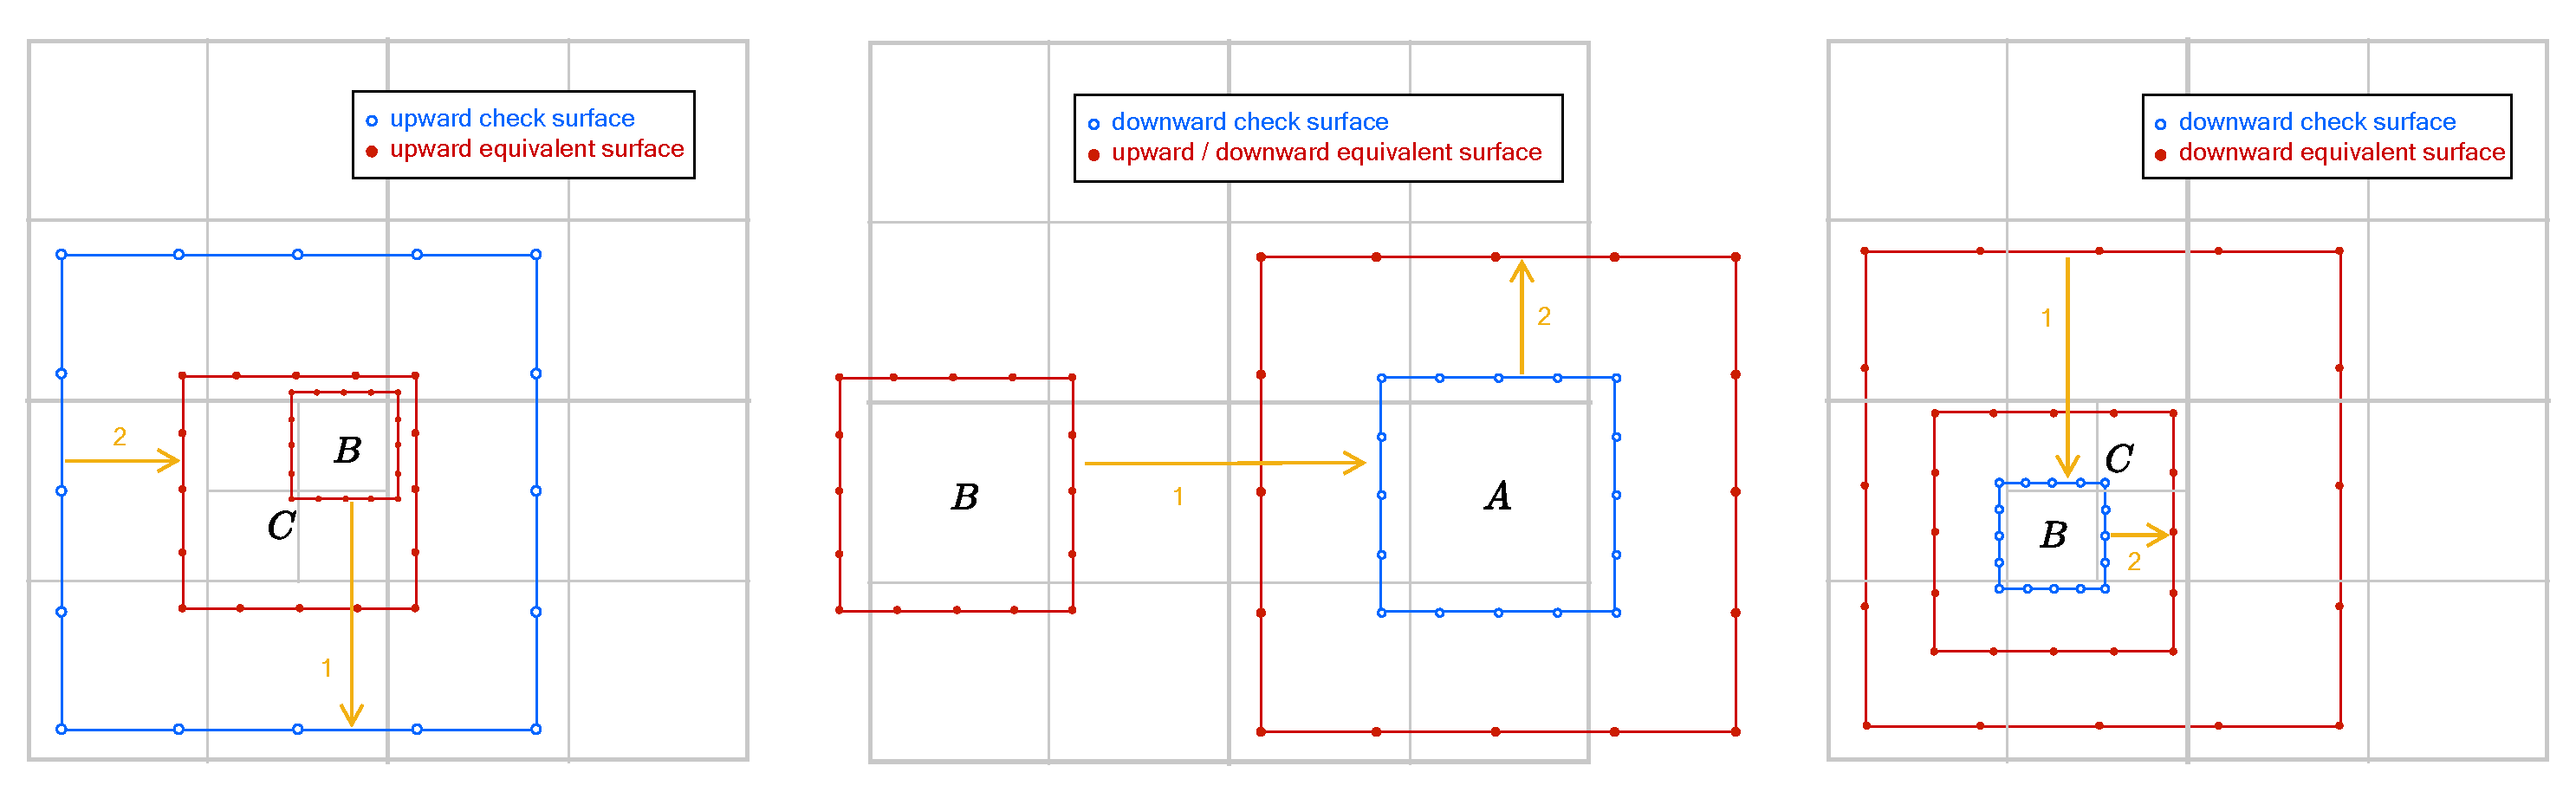
\includegraphics[width=\linewidth]{translations.pdf}
    \caption{M2M (left), M2L (middle) and L2L (right) operators in KIFMM. Node $C$ is the parent of $B$, and node $A$ is in the interaction list of $B$.}
    \label{fig:translations}
\end{figure*}

\begin{figure}
    \centering
    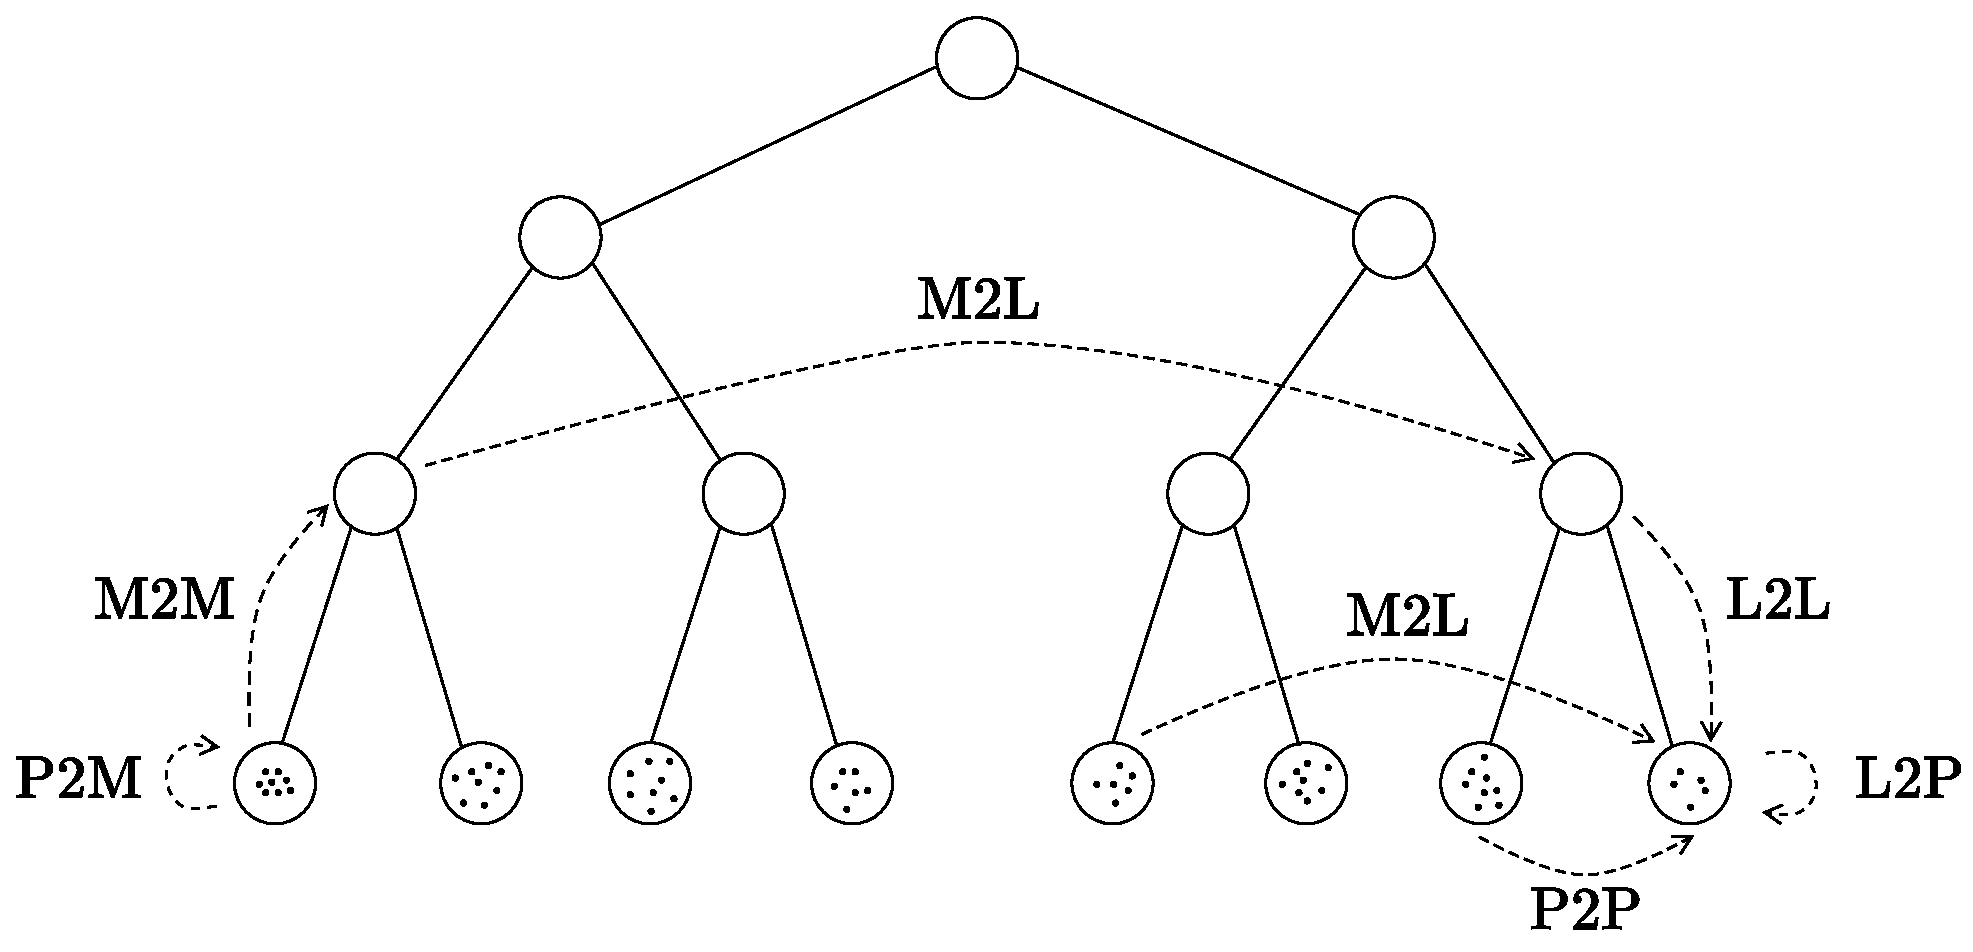
\includegraphics[width=\linewidth]{fmm_sketch.pdf}
    \caption{Sketch of FMM algorithm using a binary tree.}
    \label{fig:fmm_sketch}
\end{figure}